\section{Yocto: pour qui ? pourquoi?}

Pour construire son OS aujourd'hui, il existe de nombreux outils. Un outils (ou plutôt ensemble d'outils) très utilisé est buildroot. Mais il en exeiste plein d'autre.
Dans le monde de l'industrie le projet Yocto est de plus en plus présent et nous allons voir pourquoi.
\subsection{Les outils disponibles pour construire son OS aujourd'hui}
\paragraph{}

Comme nous l'avons dit, les outils permettant la création d'OS sont multiples.
Voici une synthèse des principaux :
\paragraph{}
Do It Yourself : limité aux cas simples
\begin{itemize} 

\item Avantage = maîtrise totale

\item Inconvénient = il faut tout faire
\end{itemize} 

\paragraph{}
Buildroot : simple mais fonctionnellement moins
riches que les autres
\begin{itemize} 

\item Adapté aux applications enfouies, pas très riches

\item Difficile de travailler en différentiel : régénération complète du
File System, pas de gestion de paquets

\item Basé sur des Makefiles
\end{itemize} 

\paragraph{}
Scratchbox : riche mais obsolète

\paragraph{}
LTIB : outil utilisé par Freescale, mais changement en
cours au profit du Yocto Project

\begin{itemize} 

\item Versions logicielles datées (host + target)

\end{itemize} 



\paragraph{}
OpenEmbedded : Ancêtre commun issu du projet Open Zaurus, toujours actif.
\begin{itemize} 

\item Base de distributions variées

\end{itemize} 
\paragraph{}
Et il en existe encore bien d'autre. Mais alors avec cette forte diversité pourquoi choisir YOCTO ?
Les avantages sont multiples bien sûr, mais le plus important est son côté modulable.
Aussi, ce projet permet de mettre en place de manière industrielle des outils de création de distribution Linux embarqué. C'est donc un projet oprmisé pour le monde de l'industrie.
En effet, du fait de l'évolution des compasants d'un système il faut avoir une certaine flexibilité sur l'OS que l'on conçoit. Yocto permet cette flexibilité.
De plus, le projet Yocto est sous l'égide de la Linux Foundation ce qui permet une certaine garantie de fonctionnement.
On voit donc un peu plus pourquoi Yocto est apprécié des industriels.
Mais comme nous l'avons vu ce projet ce distingue notamment de par sa fléxibilité.
Nous allons maintenant expliquer comment cette flexibilité est permise.





\subsection{Yocto : un fonctionnement plus flexible}
\begin{figure}[ht!]

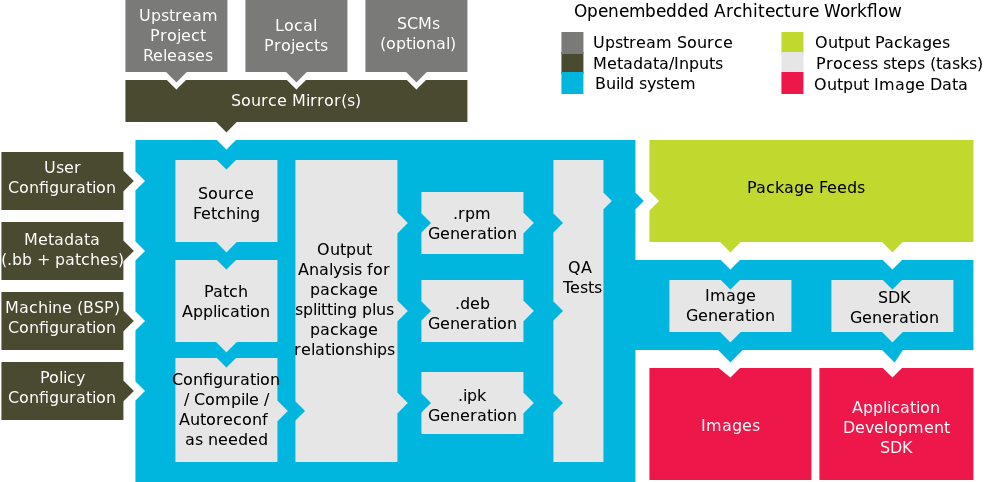
\includegraphics[width=\linewidth]{yocto.png} % Figure image 

\caption{crédit: Yocto project} % Figure caption 


\label{Project Yocto} % Label for referencing with \ref{bear} 
\end{figure}


\paragraph{}
Pour la conctruction de son OS avec Yocto, il faut choisir ces entrées.
On a bien sûr les codes sources des derniers projets visibles sur le site de yocto.
Mais le plus important étant les fichiers de configurations:
\begin{itemize} 

\item Caractéristiques de la machine cible (kernel, bootloader, format
image, tuning compilateur ...)
\item Caractéristiques de la distribution (paquets inclus, versions, choix
entre alternatives, choix libc ...)
\item Caractéristiques des layers (spécificité du projet)
\item Configuration du build : machine, distribution, layers actives, format
paquet ...

\end{itemize} 
La compilation de l'OS est réalisé par le moteur bitbake qui est une chaine de cross compilation codée en python.
Bitbake permet des sorties d'une grande modularité.
Ce qui permet d'embarquer un gestionnaire de paquets sur la cible
Il permet aussi  de travailler en différentiel pour d'éventuelles mise à jour et un enrichissement permanent.
En fait, avec bitbake l'OS se construit couche par couche.
Un jeu de recettes permet de fabriquer les paquets logiciels.
La notion de classes permet de regrouper les recettes.
Il existe aussi les méta paquets qui ont la fonction de structurer
(packagegroup)
Les dépendances entre ces paquets sont décrites dans les
recettes, ou déterminées automatiquement (librairies
partagées)
Bitbake aide aussi pour le calcul de l'arbre des dépendances pour fabriquer les
paquets dans le bon ordre.

Et c'est cette structure en couche qui permet cette flexibilité.
Possibilité de créer sa propre layer (niveau
société)
Possibilité de créer des layers par affaire ou
projet
Le but est d'optimiser la réutilisation des recettes
en évitant au maximum la duplication.
Si une même recette présente dans plusieurs
layers, c'est la layer de priorité supérieure qui
s'impose.

Et cette structure en couche permet une meilleur "réutilisabilité".
Malgrès tout ces élèments d'explication, créer son OS avec Yocto peut s'avérer difficile.
C'est pourquoi dans la prochaine partie, nous allons expliquer pas à pas la construction d'un OS avec yocto.